\usetikzlibrary{fit, positioning,backgrounds}
% Custom styles for colored borders
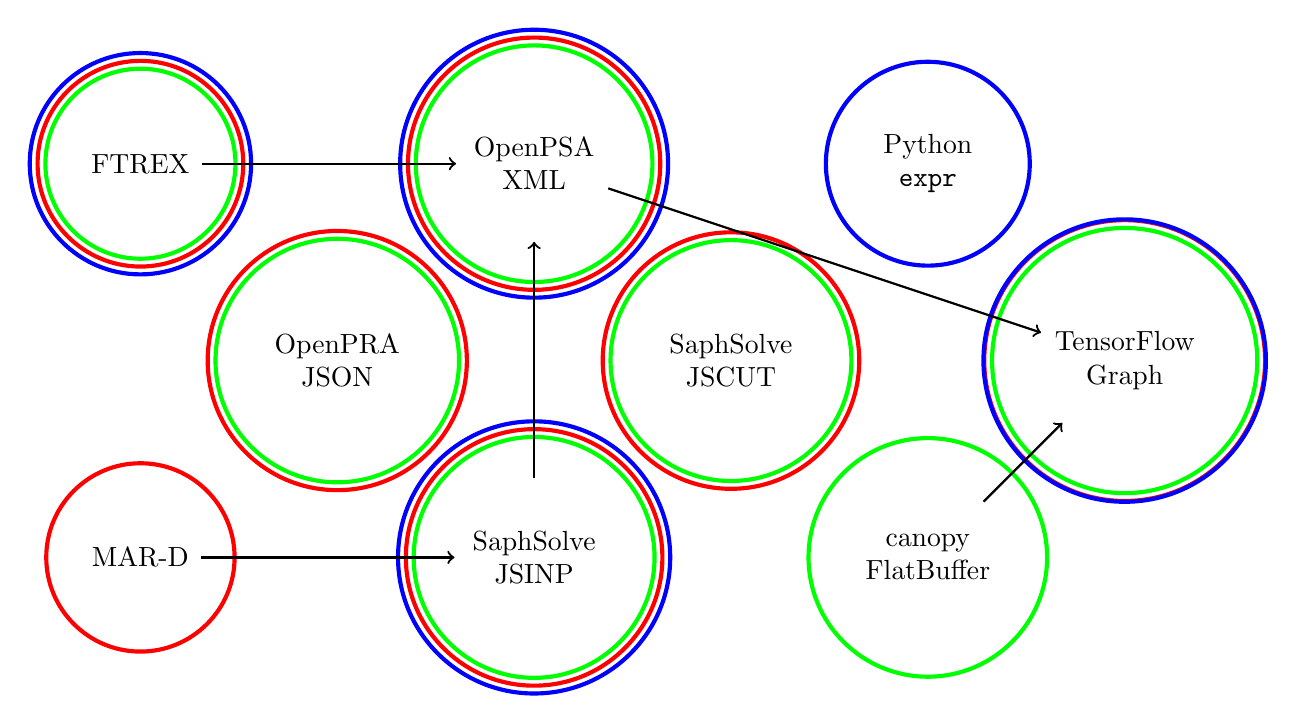
\begin{tikzpicture}[
    translation/.style={->,thick},
    schema/.style={
        circle,
        % fill=blue!10,
        minimum size=10mm,
        align=center
    },
    node distance=20mm and 30mm
]

% Nodes
\node[schema] (ftrex) at (-5,2.5) {FTREX};
\node[schema] (mard) at (-5,-2.5) {MAR-D};
\node[schema] (openpra) at (-2.5,0) {OpenPRA\\JSON};
\node[schema] (openpsa) at (0,2.5) {OpenPSA\\XML};
\node[schema] (jsinp) at (0,-2.5) {SaphSolve\\JSINP};
\node[schema] (jscut) at (2.5,0) {SaphSolve\\JSCUT};
\node[schema] (expr) at (5,2.5) {Python\\\texttt{expr}};
\node[schema] (canopy) at (5,-2.5) {canopy\\FlatBuffer};
\node[schema] (tensorflow) at (7.5,0) {TensorFlow\\Graph};

% Edges (translations)
\draw[translation] (ftrex) -- (openpsa);
\draw[translation] (mard) -- (jsinp);
\draw[translation] (jsinp) -- (openpsa);
\draw[translation] (openpsa) -- (tensorflow);
\draw[translation] (canopy) -- (tensorflow);

% Background rings
\begin{pgfonlayer}{background}
    % FTREX: readfile, writefile, programmatic
    \node[circle, draw=green, line width=1.5pt, fit=(ftrex), inner sep=2pt] {};
    \node[circle, draw=red, line width=1.5pt, fit=(ftrex), inner sep=4pt] {};
    \node[circle, draw=blue, line width=1.5pt, fit=(ftrex), inner sep=6pt] {};

    % MAR-D: writefile
    \node[circle, draw=red, line width=1.5pt, fit=(mard), inner sep=2pt] {};

    % OpenPRA: readfile, writefile
    \node[circle, draw=green, line width=1.5pt, fit=(openpra), inner sep=2pt] {};
    \node[circle, draw=red, line width=1.5pt, fit=(openpra), inner sep=4pt] {};

    % OpenPSA: readfile, writefile, programmatic
    \node[circle, draw=green, line width=1.5pt, fit=(openpsa), inner sep=2pt] {};
    \node[circle, draw=red, line width=1.5pt, fit=(openpsa), inner sep=4pt] {};
    \node[circle, draw=blue, line width=1.5pt, fit=(openpsa), inner sep=6pt] {};

    % JSINP: readfile, writefile, programmatic
    \node[circle, draw=green, line width=1.5pt, fit=(jsinp), inner sep=2pt] {};
    \node[circle, draw=red, line width=1.5pt, fit=(jsinp), inner sep=4pt] {};
    \node[circle, draw=blue, line width=1.5pt, fit=(jsinp), inner sep=6pt] {};

    % JSCUT: readfile, writefile
    \node[circle, draw=green, line width=1.5pt, fit=(jscut), inner sep=2pt] {};
    \node[circle, draw=red, line width=1.5pt, fit=(jscut), inner sep=4pt] {};

    % EXPR: programmatic
    \node[circle, draw=blue, line width=1.5pt, fit=(expr), inner sep=2pt] {};

    % CANOPY: readfile
    \node[circle, draw=green, line width=1.5pt, fit=(canopy), inner sep=2pt] {};

    % TENSORFLOW: readfile, writefile, programmatic
    \node[circle, draw=green, line width=1.5pt, fit=(tensorflow), inner sep=2pt] {};
    \node[circle, draw=red, line width=1.5pt, fit=(tensorflow), inner sep=4pt] {};
    \node[circle, draw=blue, line width=1.5pt, fit=(tensorflow), inner sep=6pt] {};
\end{pgfonlayer}

\end{tikzpicture}